\section{Motivation} \label{sec:motivation}
High level synthesis tools greatly alleviate the efforts of building BFS accelerators on FPGAs. 
Nevertheless, the performance of the resulting accelerators can be far from satisfying 
especially for irregular applications like BFS. In this section, we take our own experience 
on optimizing BFS on Alpha-Data as an example and show the challenge of 
optimizing BFS with HLS tools.

We started from basic sequential BFS algorithm for 
the HLS design. First of all, we separated the nested loop into different pipeline 
stages connected via FIFO using data flow model supported by Xilinx HLS. 
We explored all the possible pipeline combinations ranging from single-stage 
pipeline to seven-stage pipeline. With the optimized pipeline, we further 
introduced prefetch buffer to improve memory access efficiency, 
added customized cache structure for the vertex property to reduce the external 
memory accesses, hash table based redundancy removal logic to reduce the repeated 
outgoing neighboring vertices of the frontier vertices. Finally, we also tried to 
duplicate the pipeline stages for parallel processing and tuned the design parameters 
of the accelerators such as cache and prefetch buffer size. We believed 
we had tried the major design optimization methods that could be applied to the 
baseline HLS design. 

%\begin{algorithm}
%	\caption{BFS Algorithm} \label{alg:bfs}
%    \small
%	\begin{algorithmic}[1]
%		\Procedure{BFS}{}
%		\State $level[v_k] \gets -1$ where $v_k \in V$
%		\State $level[v_s] \gets 0$
%		\State $current\_level \gets 0$
%		\State $frontier \gets v_s$
%
%        \While {$!frontier.empty()$} 
%
%		\For{$v \in V$}
%		\If{$level[v] == current\_level$}
%		\State $frontier \gets v$
%		\EndIf
%		\EndFor
%
%		\For{$v \in frontier$}
%		\State $S \gets {n \in V | (v, n) \in E}$
%		\For {$n \in S$}
%		\If {$level[n] == -1$}
%		\State $level[n] \gets current\_level + 1$
%		\EndIf
%		\EndFor
%		\EndFor
%		\State $current\_level \gets current\_level + 1$
%		\EndWhile
%		\EndProcedure
%	\end{algorithmic}
%\end{algorithm}

We measured the performance of the accelerator with a set of representative graphs 
including Youtube, Live Journal, Orkut and two R-MAT graphs. Details about the 
graph benchmark can be found in Table \ref{tab:graph} in the experiment section. 
Figure \ref{fig:opt-performance} presents the normalized performance
when different optimization techniques are gradually applied to the naive baseline design.
It can be found that the resulting BFS accelerator achieves up to 70X performance speedup
compared to the baseline design. It indicates that the HLS optimizations help improve the 
performance significantly. However, when the accelerator is compared to the existing 
handcrafted design reported in prior work \cite{betkaoui2012reconfigurable}, 
\cite{attia2014cygraph}, \cite{zhang2017boosting}, \cite{nurvitadhi2014graphgen},
\cite{dai2016fpgp}, it remains far from satisfying. On the graph benchmark in Table \ref{tab:graph}, 
the average performance is 38.8 MTEPS, which is 10X to 20X less than the typical handcrafted 
design as shown in Table \ref{tab:compare} in the experiment section.

\begin{figure}
	\center{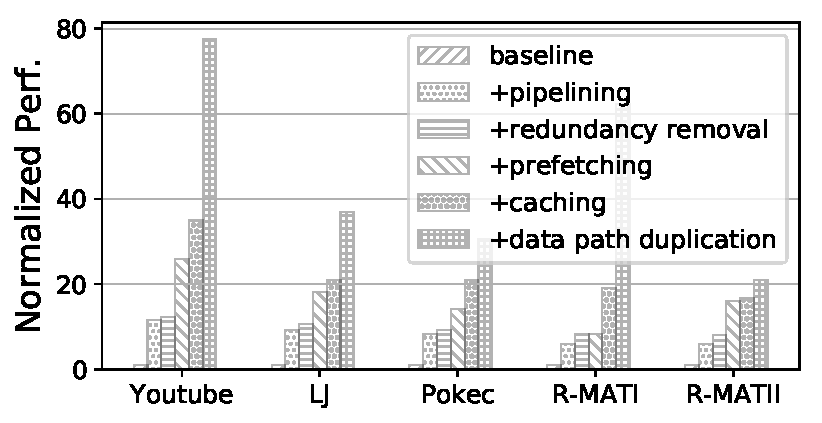
\includegraphics[width=0.85\linewidth]{opt-performance}}
    \caption{The normalized performance of an HLS based BFS accelerator with various optimizations on Alpha-Data}
\label{fig:opt-performance}
\vspace{-1em}
\end{figure}

While the baseline design could be created using HLS in around an hour, optimizing the 
HLS design took much longer time. The optimization took an experienced hardware designer 
with basic high level synthesis knowledge up to months, though most of time was 
spent on implementing the large amount of combined optimization methods and cumbersome
debugging when software simulation passed but the accelerator got stalled 
during hardware execution. In general, it can be found that developing an optimized BFS 
accelerator using HLS tools remains a challenging task and will be even more difficult for 
designers without much hardware knowledge. Meanwhile, we also notice that the benefits of 
the HLS design is also attractive. Despite the difference between Xilinx HLS 
and Intel OpenCL, porting the design to FPGA devices of different vendors is trivial. 

Therefore, we argue that it is beneficial to have the experienced designers to explore the HLS based 
application acceleration and provide the HLS solutions to more users without hardware 
experiences. This motivates us to focus on the high-level BFS accelerator optimization
and offer open-sourced BFS design with both the near handcrafted performance and 
the software-like flexibility.

